%% Internal report for Jan Streffing and Thomas Jung (not for the paper), 2026-11-10.
%% How Fig. 3c and 3d of the Dunkelflaute paper (paper/figures/fig_mechanism.tex) are obtained and how robust they are.
%% Sources (analysis repo /work/ab0246/a270092/software/dark-doldrums-project, all under dunkelflaute/):
%%   [RS]  results/regimes/regime_summary.json               (scripts/regimes/regime_analysis.py)
%%   [RP]  results/regimes/regime_patterns.npz               (regime_analysis.py)
%%   [DR]  results/regimes/regime_decomposition_robustness.json/.npz (scripts/regimes/regime_decomposition_robustness.py, new)
%%   [GR]  results/regimes/regime_G_robustness.json          (scripts/regimes/regime_G_robustness.py)
%%   [ED]  results/regimes/eof_diagnostics/eof_diagnostics.json and *.png (scripts/regimes/eof_diagnostics.py)
%%   [GS]  results/regimes/geostrophic_summary.json          (scripts/regimes/geostrophic.py)
%%   [TC]  results/regimes/transfer_checks.json              (scripts/regimes/transfer_checks.py)
%%   [PK]  results/regions/region_per_K_summary.json         (scripts/regions/region_per_K.py)
%%   [MN]  docs/methods_notes.md Sect. 13, 13b
%% Figures in figs/ and table bodies in tables/ are written by scripts/regimes/regime_checks_report_figs.py (new).
%% Build: module load texlive/live2025-gcc-13.3.0; latexmk -pdf regime_checks.tex
\documentclass[10pt,a4paper]{article}
\usepackage[margin=2.2cm]{geometry}
\usepackage[T1]{fontenc}
\usepackage{lmodern}
\usepackage{amsmath}
\usepackage{graphicx}
\usepackage{booktabs}
\usepackage{makecell}
\usepackage{array}
\usepackage{flafter}
\usepackage{xcolor}
\usepackage[font=small,labelfont=bf]{caption}
\usepackage[hidelinks]{hyperref}
\setlength{\parskip}{3pt}
\setlength{\emergencystretch}{2em}
\renewcommand{\topfraction}{0.9}\renewcommand{\bottomfraction}{0.8}
\renewcommand{\textfraction}{0.07}\renewcommand{\floatpagefraction}{0.85}
\setcounter{topnumber}{3}\setcounter{totalnumber}{5}
\renewcommand{\cellalign}{cc}
\newcommand{\lam}{\lambda}
\makeatletter\let\tabinput\@@input\makeatother  % primitive input, so that \bottomrule may follow inside tabular

\title{Figure 3c and 3d of the Dunkelflaute paper:\\ how they are made and how robust they are}
\author{Internal note for Jan Streffing and Thomas Jung}
\date{10 November 2026}

\begin{document}
\maketitle

\section{Summary}

%% [DR] reproduce max |d| <= 1.1e-15; [GR] ScBL p, CMIP6 counts; [AT] regime_G_attribution.json.
The question was whether the geostrophic speed $G$ really weakens this clearly within the weather regimes.
It does.
Single winters are noisy, but over decades the weakening under Scandinavian blocking (ScBL) stands out in every run and
in nearly every CMIP6 model.
We rebuilt Fig.~3c and 3d from the daily data, reproduced the stored numbers to machine precision, and tested both
panels against a bootstrap over winters and against unforced variability in the 147-winter constant-forcing control of
the 100\,km run.
\begin{itemize}\setlength{\itemsep}{1pt}
\item The within-regime term of Fig.~3c lies outside every placement of the control null in all four runs.
      The regime-frequency term is small and cannot be told apart from zero.
\item Under ScBL, $G$ weakens beyond the null in all four runs and beyond the winter-to-winter variability in 18 of 20 CMIP6
      models, and all 20 agree on the sign.
\item The weakening sits in the weather systems, whose pressure gradients fall at nearly unchanged amplitude.
      The mean pressure field does not cause it, since its gradient over the sector strengthens.
\item We found no earlier study with this result for wind droughts.
\end{itemize}

\section{From daily pressure to regimes}
\label{sec:regimes}

%% [MN] 13; [RS] explained_variance (first 10: 0.82), era5.freq.
The input is daily-mean sea-level pressure (msl) on a 2.5$^\circ$ grid over 20--80$^\circ$N and 80$^\circ$W--40$^\circ$E,
each value the mean of all native points within the grid box.
The regimes are defined on ERA5 alone.
We removed a mean and three annual harmonics from the 9976 September-to-March days of 1979/80--2024/25, computed EOFs,
and clustered the first 10 principal components, which explain 82\,\% of the variance, into four regimes with
$k$-means.
Model days are not clustered.
Their anomalies from the seasonal cycle of the comparison's control are projected on the ERA5 EOFs, and each day goes to
the nearest ERA5 centroid.

%% [ED] summary_ours.png; assigned ctlclim r >= 0.99 controls, >= 0.93 futures; CMIP6 hist >= 0.977.
The ERA5 patterns are a fair basis for the models (Fig.~\ref{fig:eofsum}).
The first three model EOFs match ERA5 with pattern correlations of 0.87 to 0.99.
Clustering each run on its own gives unstable centroids on 10 to 17 winters, as it does for ERA5 sub-periods of the
same length, which is why we assign model days to the ERA5 centroids instead.
The composites of the assigned days reproduce the ERA5 centroids with $r\ge0.99$ in the controls and $r\ge0.98$ in all
CMIP6 historical runs.

\begin{figure}[!tbp]
\centering
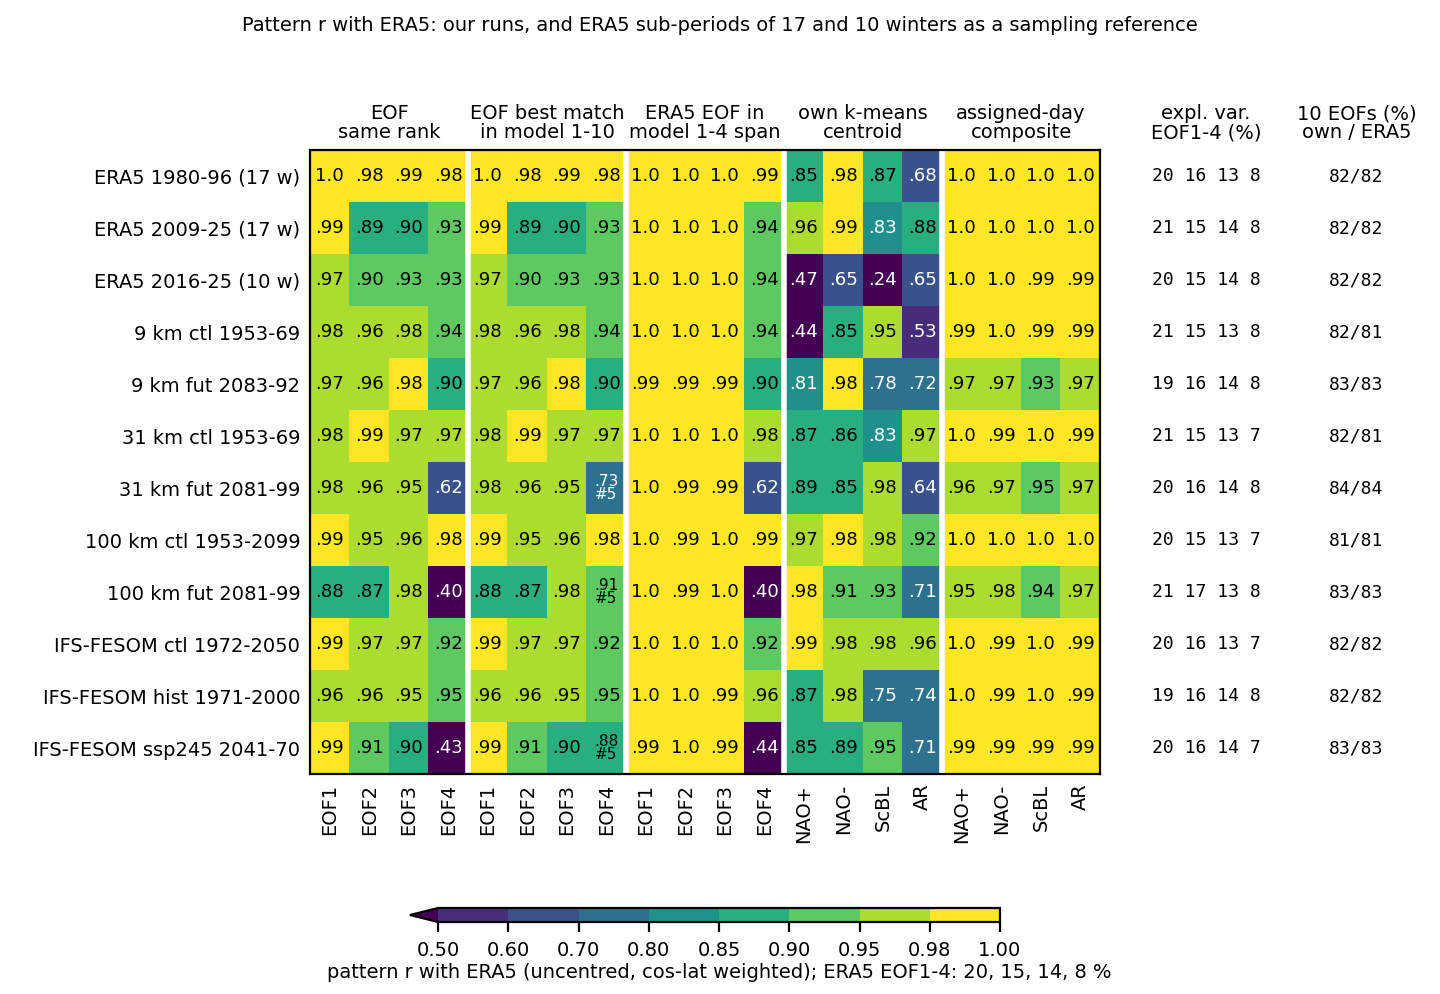
\includegraphics[width=0.92\textwidth]{../../results/regimes/eof_diagnostics/summary_ours.png}
\caption{Pattern correlation with ERA5 for our runs and for ERA5 sub-periods of 17 and 10 winters. The paper uses only
the last block, the composites of the assigned days.}
\label{fig:eofsum}
\end{figure}

\section{Figure 3c step by step}
\label{sec:3c}

%% [MN] 10c/13, region_events.py: WIN = 8 six-hourly steps, TARGET 5.0.
A low-wind event is a spell in which the 48\,h mean of the region's wind capacity factor stays below a threshold.
The threshold is set separately in each region and run so that the control has five events per winter, which makes
it a percentile of that run's own distribution, and the future is counted at the same threshold.
Each event takes the regime that covers most of its days.
For one region and period, let $f_k$ be the regime-$k$ days per winter and $\lam_k$ the events per regime-$k$ day, so that
the events per winter are $e=\sum_k f_k\lam_k$.
The change from control to future splits exactly into
\begin{equation}
\Delta e \;=\; \underbrace{\sum_k \lam_k^{\mathrm{ctl}}\,\bigl(f_k^{\mathrm{fut}}-f_k^{\mathrm{ctl}}\bigr)}_{\text{frequency term}}
\;+\; \underbrace{\sum_k f_k^{\mathrm{fut}}\,\bigl(\lam_k^{\mathrm{fut}}-\lam_k^{\mathrm{ctl}}\bigr)}_{\text{within-regime term}} .
\label{eq:dec}
\end{equation}
Both terms are computed per region, averaged over the eight European regions, and divided by the global-mean warming
$\Delta T$ of the comparison.

%% [DR] runs.9km.regions.DE: lam100 ScBL 4.52 -> 6.48, f 59.8 -> 50.9; total 1.5 = -0.453 + 1.953.
Table~\ref{tab:example} goes through Germany at 9\,km.
ScBL produces the most events per regime day, and under warming its rate rises from 4.5 to 6.5 events per 100 days.
Its within-regime part is the future number of ScBL days times this rise, about one event per winter.
Its frequency part is the control rate times the loss of nine ScBL days, about $-0.4$.
Summed over the four regimes, Germany gains 1.5 events per winter, a within-regime gain of 2.0 of which the
frequency term takes back 0.45.

\begin{table}[!tbp]
\centering\small
%% Body: tables/example_DE_9km.tex from [DR] runs.9km.regions.DE.
\caption{Worked example, Germany at 9\,km, control 1953--1969 against future 2083--2092. $f_k$ in regime days per
winter, $e_k$ in events per winter, $\lam_k$ in events per 100 regime days, and the two terms of Eq.~\ref{eq:dec} in
events per winter per K.}
\label{tab:example}
\begin{tabular}{lrrrrrrrr}
\toprule
& \multicolumn{2}{c}{$f_k$} & \multicolumn{2}{c}{$e_k$} & \multicolumn{2}{c}{$100\,\lam_k$} & frequency & within \\
\cmidrule(lr){2-3}\cmidrule(lr){4-5}\cmidrule(lr){6-7}
regime & ctl & fut & ctl & fut & ctl & fut & per K & per K \\
\midrule
\tabinput tables/example_DE_9km.tex 
\bottomrule
\end{tabular}
\end{table}

%% [DR] n_boot 5000; null placements 14762, 12656, 129 (rest vs 19), 1560.
The bootstrap resamples whole winters, independently in control and future and with the same winters in every region.
The null places two disjoint blocks with the comparison's numbers of winters in all possible positions within the
147-winter control and treats the second block as the future.
The within-regime term exceeds every placement of the null in all four runs (Table~\ref{tab:terms},
Fig.~\ref{fig:decboot}).
The frequency term is negative in all four runs, and its bootstrap range includes zero in all four.
%% [DR] within_k / within: 40, 61, 33, 54 %; ScBL part p <= 0.015; sensitivity max 0.015.
ScBL carries the largest share of the within-regime term in three of four runs and is significant in all four.
Splitting tied events between regimes or using the symmetric form of Eq.~\ref{eq:dec} shifts the terms by at most
0.015 events per winter per K.

\begin{table}[!tbp]
\centering\footnotesize\setlength{\tabcolsep}{3pt}
%% Body: tables/terms.tex from [DR] runs.*.
\caption{Terms of Fig.~3c, 8-region mean in events per winter per K, with the bootstrap 5--95\,\% range below each value
and the one-sided $p$ of the control null. The last column counts the regions with a positive within-regime term.}
\label{tab:terms}
\begin{tabular}{lrcclclclc}
\toprule
& & & \multicolumn{2}{c}{total} & \multicolumn{2}{c}{frequency term} & \multicolumn{2}{c}{within-regime term} & \\
\cmidrule(lr){4-5}\cmidrule(lr){6-7}\cmidrule(lr){8-9}
run & $\Delta T$ (K) & winters & \makecell{value\\5--95\,\%} & $p$ & \makecell{value\\5--95\,\%} & $p$ & \makecell{value\\5--95\,\%} & $p$ & $>0$ \\
\midrule
\tabinput tables/terms.tex 
\bottomrule
\end{tabular}
\end{table}

\begin{figure}[!tbp]
\centering
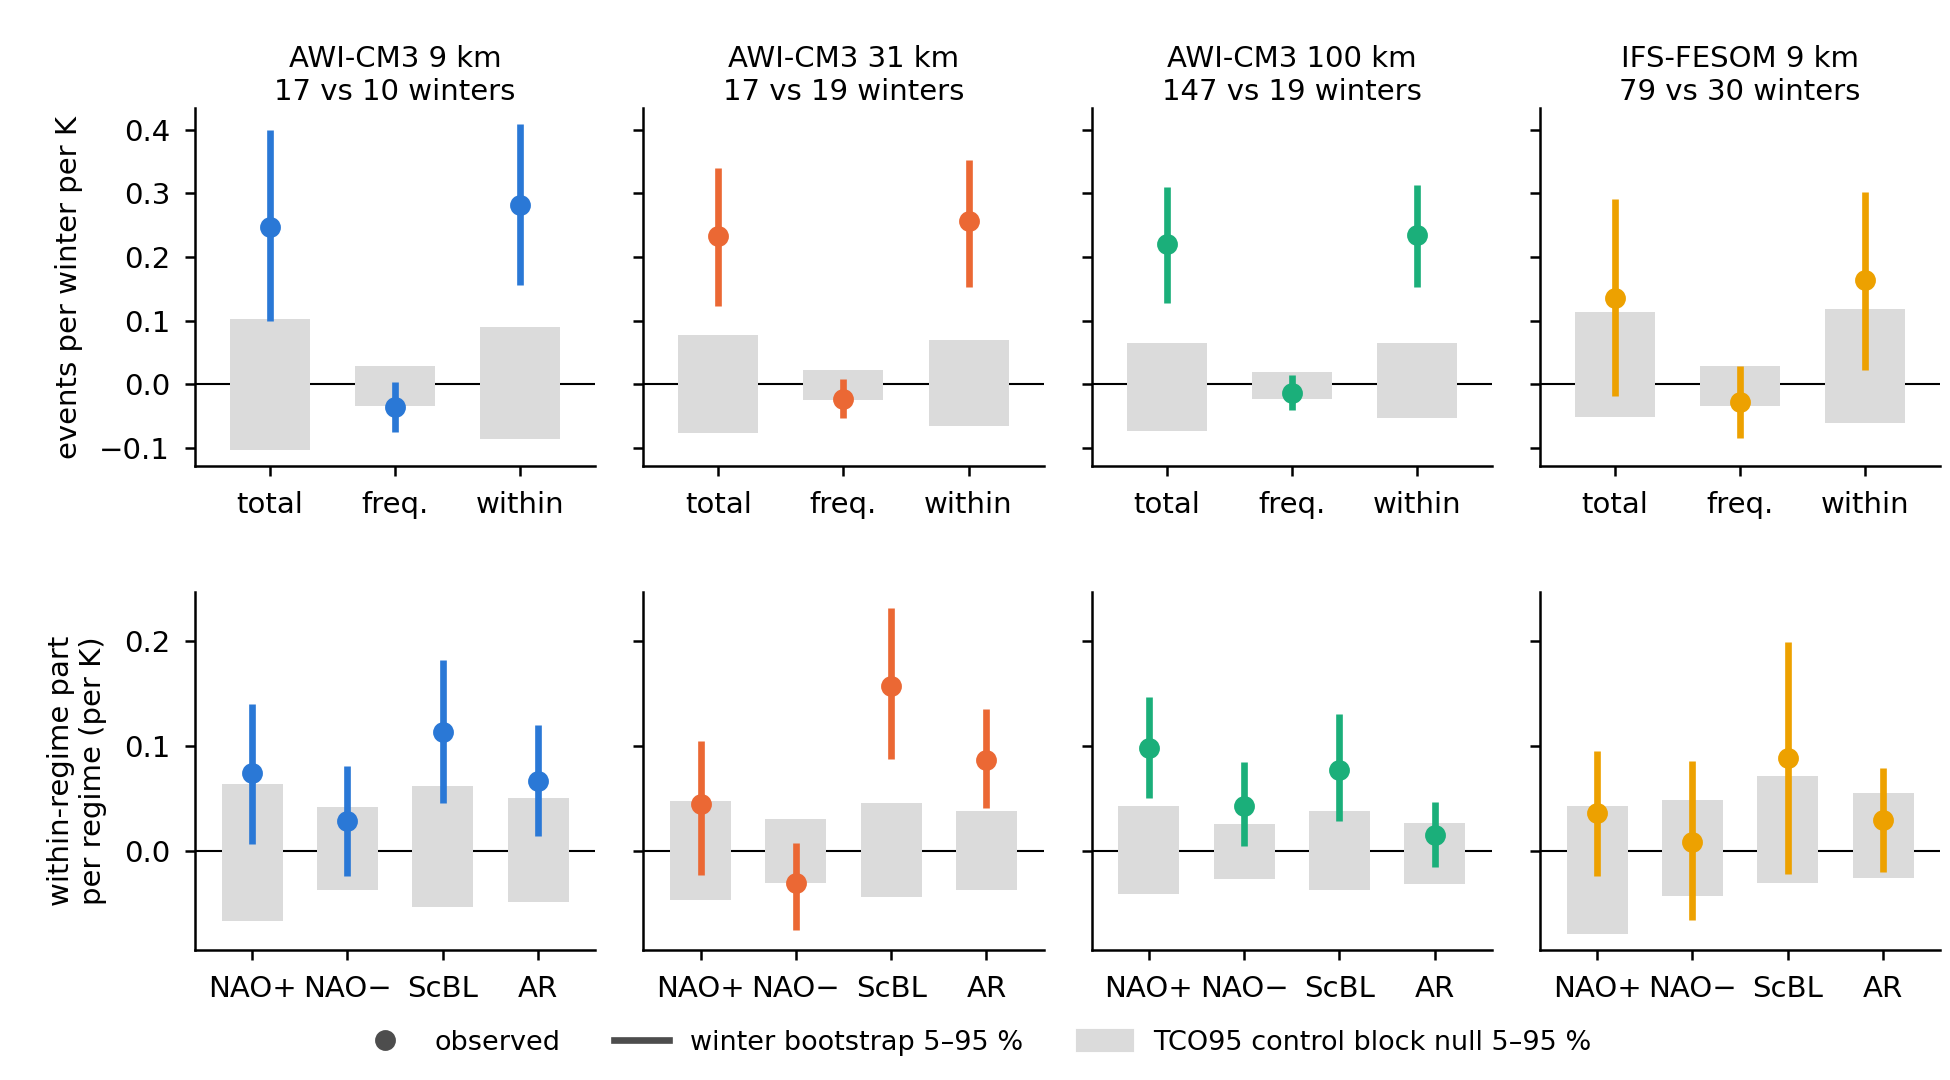
\includegraphics[width=0.92\textwidth]{figs/decomp_boot_null.png}
\caption{Robustness of Fig.~3c. Top, the total and the two terms of each run. Bottom, the within-regime term split by
regime. Dots are the observed values, bars the winter bootstrap 5--95\,\% range, and grey boxes the 5--95\,\% range of
the block null from the 147-winter 100\,km control.}
\label{fig:decboot}
\end{figure}

\section{Figure 3d step by step}
\label{sec:3d}

%% [MN] 13b; geostrophic.py: RHO 1.25, centred differences.
From the daily msl $p$ we computed $G=|\nabla p|/(\rho f)$ with centred differences, $\rho=1.25$\,kg\,m$^{-3}$ and
$f=2\Omega\sin\varphi$, averaged over each region box.
For each region and regime we compared the mean $G$ of all regime days in future and control, averaged the change over
the eight regions, and expressed it per kelvin as $100\,\bigl(\exp[\ln(1+\Delta G/100)/\Delta T]-1\bigr)$.
Our runs use the msl of the regime analysis, and CMIP6 uses daily psl interpolated bilinearly onto the same 2.5$^\circ$
grid.
%% [DR] G_footing: largest |diff| 0.225 %/K.
On the bilinear footing our values change by at most 0.23\,\% per K.

%% [GR] ScBL block null p 0 of all placements, 100 km 30 vs 19 p 0.0122; sd 4-8 %; CMIP6 ScBL 20 negative, 18 below zero.
Under ScBL the weakening exceeds every placement of the null in all four runs (Fig.~\ref{fig:Gboot}, Table~\ref{tab:G}).
In CMIP6 all 20 models weaken under ScBL, and in 18 the bootstrap range lies below zero.
The other regimes weaken less and are significant only in some runs.
A single winter is noisy, with a standard deviation of 4 to 8\,\% in winter-mean ScBL $G$, so the signal emerges only
over decades.
Labelling the future with its own seasonal cycle, or keeping only the ScBL days closest to the centroid, leaves the
weakening in place.

\begin{figure}[!tbp]
\centering
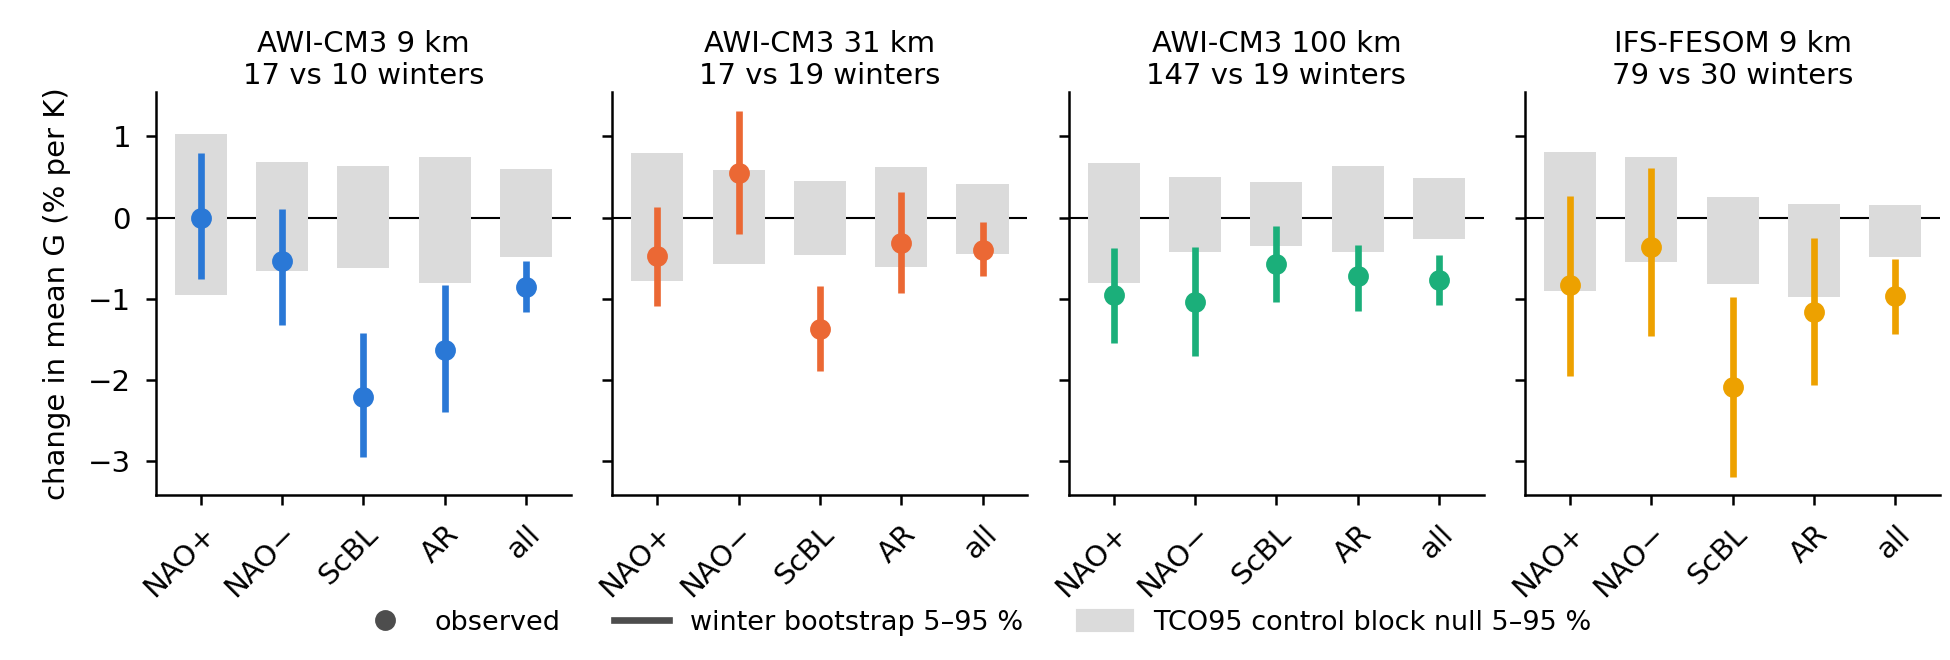
\includegraphics[width=0.92\textwidth]{figs/G_boot_null.png}
\caption{Change in mean $G$ within each regime and over all days, \% per K, eight regions. Dots, bootstrap bars and
null boxes as in Fig.~\ref{fig:decboot}.}
\label{fig:Gboot}
\end{figure}

\begin{table}[!tbp]
\centering\footnotesize\setlength{\tabcolsep}{3pt}
%% Body: tables/G_per_regime.tex from [GR] and [DR] G_footing.
\caption{Change in mean $G$ within regimes, \% per K. For our runs the value of Fig.~3d with its bootstrap 5--95\,\%
range, the null $p$, and the value on the bilinear CMIP6 footing (``bil.''). For CMIP6 the median and the 10--90\,\%
range of 20 models, the number of models with a negative change and the number whose bootstrap range lies below zero.}
\label{tab:G}
\begin{tabular}{lccccc}
\toprule
regime & 9 km & 31 km & 100 km & IFS-FESOM & CMIP6 \\
\midrule
\tabinput tables/G_per_regime.tex 
\bottomrule
\end{tabular}
\end{table}

\section{Why the models agree, and whether this is known}
\label{sec:lit}

%% [AT] results/regimes/regime_G_attribution.json (scripts/regimes/regime_G_attribution.py); reproduces stored G change to 2e-13 %.
We split each day's pressure field into the seasonal cycle of its period and the anomaly, and recomputed $G$ with the
two swapped between control and future.
The weakening comes almost entirely from the anomalies, the weather, and this anomaly term is negative in every regime,
every run and all 20 CMIP6 models (Fig.~\ref{fig:attribution}).
The mean pressure field does not explain it, since its north--south gradient over the sector strengthens as pressure
falls over the Arctic and Nordic seas.
Under ScBL this background term is close to zero, whereas in the other regimes it is positive and offsets part of the
weakening, which is why blocking shows the clearest net signal.
The blocking high itself hardly changes in peak, extent or position.
What weakens is the gradient of the day-to-day deviations from the regime pattern, at nearly unchanged amplitude, so the
synoptic disturbances become broader and smoother.

\begin{figure}[!tbp]
\centering
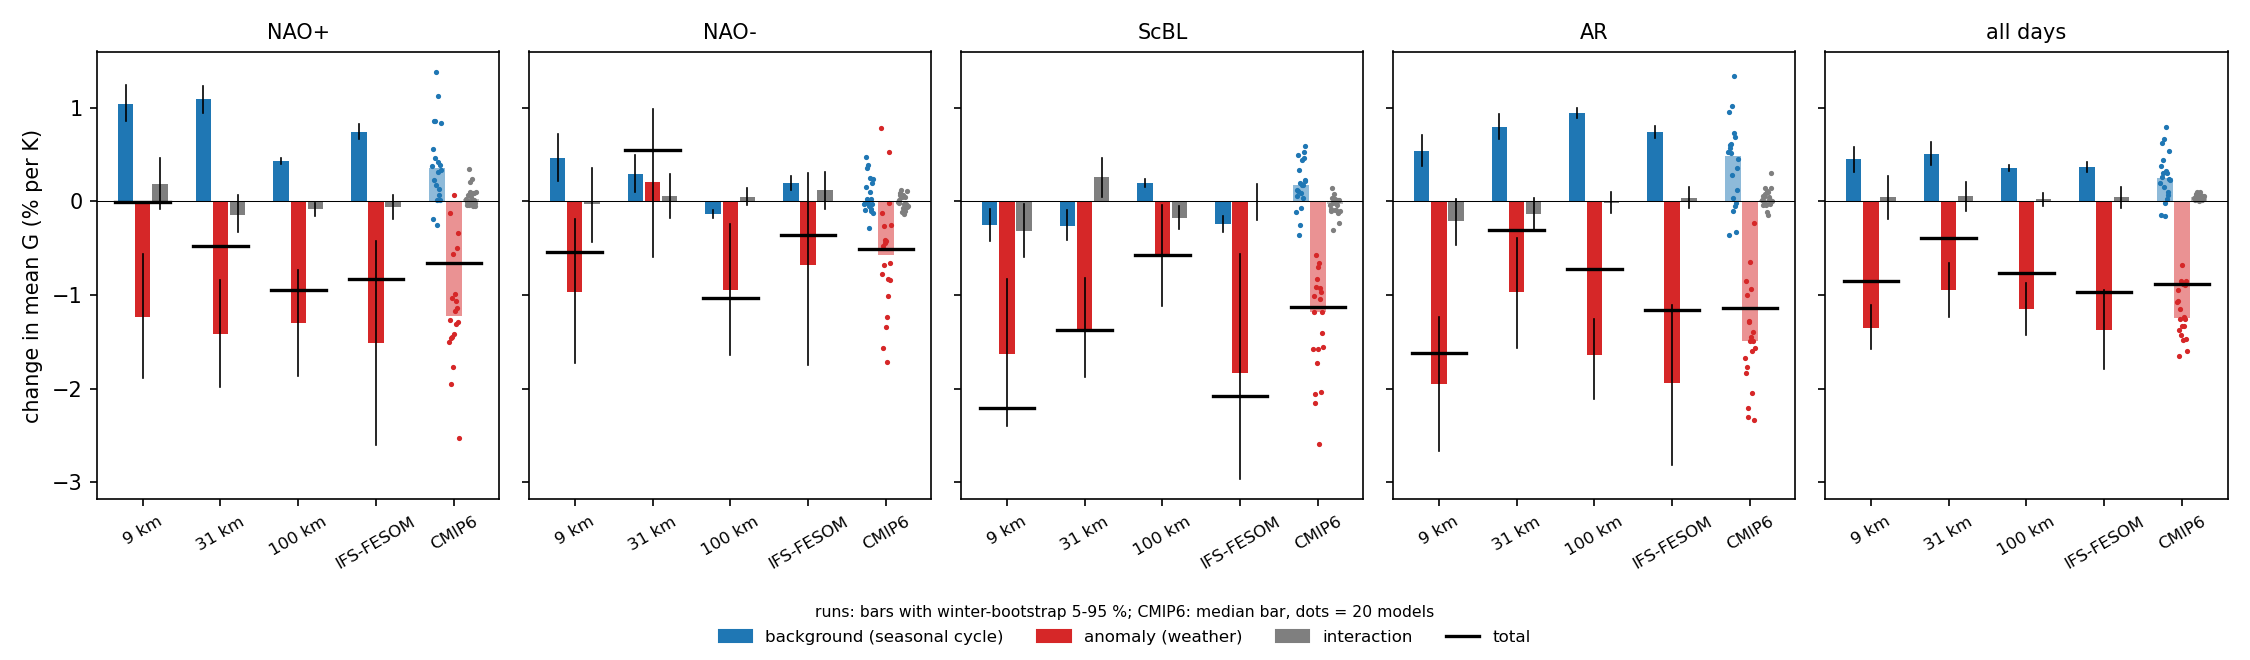
\includegraphics[width=\textwidth]{figs/attribution_per_K.png}
\caption{Change of mean $G$ per regime split into a part from the seasonal cycle (background, blue), from the anomalies
(weather, red), and their interaction (grey). Black bars are the totals of Fig.~3d. Our runs with winter-bootstrap
5--95\,\% ranges, CMIP6 as median bars with one dot per model.}
\label{fig:attribution}
\end{figure}

%% Literature search 2026-11-10 (agent, web).
We found no study that splits projected changes in wind droughts into a regime-frequency and a within-regime part, and
none that shows weaker pressure gradients within blocking across models and per kelvin of warming.
For precipitation, the change of the weather within fixed regimes outweighs the change of their frequency
\cite{fischer2025,grams2026}.
Broader disturbances match the projected increase of the eddy length scale under warming \cite{kidston2011}.
A weaker low-level temperature gradient between equator and pole damps synoptic anomalies in idealised models
\cite{hassanzadeh2014,schneider2015} and tracks projected European offshore wind \cite{wohland2022}, and the
geostrophic wind from sea-level pressure declines over the Northeast Atlantic in 32 CMIP6 models \cite{krieger2026}.
Neither the mean pressure gradient nor a regional temperature contrast explains the spread between our models
($|r|\le0.26$), so the weakening is a robust change of the weather systems whose cause remains open.

\section{Changes made in the paper}
\label{sec:text}

The paper now states the robust result plainly and leaves the tests to the Supplement.
The change in events is almost entirely a change within regimes, well beyond unforced variability, and under ScBL $G$
falls in all 20 CMIP6 models and in all four of our runs.
The Discussion says that the weakening sits in the weather systems and not in the mean state, consistent with broader
eddies, and that its cause remains open.

\begin{thebibliography}{99}\small
\bibitem{fischer2025} Fischer, M., et al. (2025), Weather Clim. Dynam. 6, 1027, doi:10.5194/wcd-6-1027-2025.
\bibitem{grams2026} Grams, C. M. (2026), Weather Clim. Dynam. 7, 1641, doi:10.5194/wcd-7-1641-2026.
\bibitem{hassanzadeh2014} Hassanzadeh, P., Kuang, Z., and Farrell, B. F. (2014), Geophys. Res. Lett. 41, 5223, doi:10.1002/2014GL060764.
\bibitem{kidston2011} Kidston, J., Vallis, G. K., Dean, S. M., and Renwick, J. A. (2011), J. Clim. 24, 3764, doi:10.1175/2010JCLI3738.1.
\bibitem{krieger2026} Krieger, D., and Weisse, R. (2026), Earth Syst. Dynam. 17, 1, doi:10.5194/esd-17-1-2026.
\bibitem{schneider2015} Schneider, T., Bischoff, T., and P{\l}otka, H. (2015), J. Clim. 28, 2312, doi:10.1175/JCLI-D-14-00632.1.
\bibitem{wohland2022} Wohland, J. (2022), Environ. Res. Lett. 17, 124047, doi:10.1088/1748-9326/aca77f.
\end{thebibliography}

\end{document}
